% template for random notes
% Tinghui Zhou
\documentclass[12pt]{article}
\usepackage{parskip}

\usepackage{amsmath,amssymb,graphicx,fullpage,subfigure,color}
\usepackage{algorithm}
\usepackage{algorithmic}

%roman font math operators
\DeclareMathOperator\aut{Aut}

\newcommand{\bx}{\mathbf{x}}
\newcommand{\bc}{\mathbf{c}}
\newcommand{\bw}{\mathbf{w}}
\newcommand{\br}{\mathbf{r}}
\newcommand{\cB}{\mathcal{B}}
\newcommand{\tx}{\tilde{x}}


% custom line spacing ----------------------------------------------------------
\usepackage{setspace}
%\onehalfspacing % one-and-a-half spacing
%\doublespacing % double spacing
%\setstretch{1.25} % custom line spacing

% begin document %%%%%%%%%%%%%%%%%%%%%%%%%%%%%%%%%%%%%%%%%%%%%%%%%%%%%%%%%%%%%%%
\begin{document}

\title{title}
\author{Tinghui Zhou}
\date{}

\maketitle
\section{Introduction}
The proposed approach consists of two major components: 1) providing an efficient and effective data description scheme based on the idea of Minimum Enclosing Balls (MEBs); 2) developing a new SVM variant (referred as Ball SVM for now) that is suitable for learning from data described by the MEBs. 

One application of this approach is a much faster version of the image matching framework proposed in~\cite{shrivastava11}. As pointed out in the paper, a big limitation of their approach is the speed, since ``it requires training an SVM (with hard-negative mining) at query time ... too slow for many practical applications...". However, noting that the negative set in their case remains the same for all query images, an interesting question would be: is it possible to describe the negative set using an alternative representation such that it's efficient to be trained on? To do that, we propose a data description scheme using a set of MEBs, which tries to characterize the data with an efficient representation that can be utilized by our proposed SVM variant at query time.

Several benefits of this approach:
\begin{itemize}
\item Less memory storage. The negative set can be discarded once its corresponding MEBs are extracted.
\item Faster SVM training at query time. Originally the hard-negative mining needs to be performed over millions of image patches. With our approach, the size of negative set reduces to the number of MEBs, which would be several orders of magnitude smaller.
\end{itemize}

\section{Data description with Minimum Enclosing Balls}
In this section, we describe a method for data description using a set of Minimum Enclosing Balls (MEBs). 

\subsection{Problem Formulation}
Suppose we are given a set of data points $X = \{x_1, \ldots, x_N \}$. The goal is to find a set of balls $B = \{ (c_1, r_1), \ldots, (c_K, r_K) \}$, with $c_k$ and $r_k$ denote the center and radius of the $k$-th ball respectively, such that they enclose as many data points with as little volume as possible. 

To fit a MEB to each cluster, we use the method proposed by Tax and Duin~\cite{tax04}, where they solve this problem via a formulation similar to Support Vector Classifier:

\begin{align}
\min_{c,r} ~& r^2 + C\sum_i \xi_i \nonumber\\
\text{s.t.} ~& \| x_i - c \|^2 \le r^2 + \xi_i, ~\xi_i \ge 0~ ~\forall i
\label{eq:svdd_org}
\end{align}

\subsection{Solving SVDD with gradient descent}
\label{sec:svdd}
The SVDD objective given in Eq.~\ref{eq:svdd_org} can also be formulated as follows:
\begin{equation}
\min_{c,r} ~r^2 + C\sum_i \max(0, \| x_i - c\|^2 - r^2).
\end{equation}
Let $F$ denote the corresponding objective function. We minimize $F$ by iteratively updating $r$ and $c$. Specifically, the gradient over $c$ given fixed $r$ is given by
$$
\frac{\partial F}{\partial c} = C\sum_i g_c(x_i),
$$
where
$$
g_c(x_i) =
  \begin{cases}
   0 & \text{if } \| x_i - c\|^2 - r^2 \le 0  \\
   2(c - x_i) & \text{otherwise}.
  \end{cases}
$$
Similarly, the gradient over $r$ given fixed $c$ is 
$$
\frac{\partial F}{\partial r} = 2r + C\sum_i g_r(x_i),~\label{eq:grad_r}
$$
where
$$
g_r(x_i) =
  \begin{cases}
   0 & \text{if } \| x_i - c\|^2 - r^2 \le 0  \\
   -2r & \text{otherwise}.
  \end{cases}
$$
Note that in Page 5 of~\cite{tax04}, it's claimed that $C \ge 1$ indicates the hard-margin solution. This is because if there's $\ge 1$ points that are not enclosed, the gradient over $r$ as in Eq.~\ref{eq:grad_r} will be negative. So $r$ will become larger and larger until it can enclose all the points. In other words, the valid range for $C$ is $(0, 1)$.

\section{Ball SVM}
Now we introduce an SVM variant, referred as Ball SVM, which finds the separating hyperplane with maximum margin for data points described by MEBs. We shall see later that SVM turns out to be a special case of Ball SVM. 

Let the training data be $D = \{\bc_k, r_k, n_k, y_k\}_{k=1,\ldots,K}$, where $\bc_k$ is the center of the ball, $r_k$ is its corresponding radius, $n_k$ is the number of points enclosed by the ball, and $s_k$ equals to $1$ if the ball encloses positive points and $0$ otherwise. Our goal is to find a hyperplane $\bw$ that separates the positive and negative balls with maximum margin. First, we define the distance from a ball to the hyperplane as $d_k = \frac{y_k(\bw^{\top}\bc_k + b)}{\|\bw\|} - r_k$, i.e. the distance from the center to the hyperplane minus the radius.  Following the standard SVM derivation in~\cite{prml}, we would like to find a $\bw$ such that $d_k > 0$ for all $k$, and the margin in this case is given by $\min_k d_k$, i.e. the distance from the closest ball to the hyperplane. Therefore, our goal of finding a maximum margin solution can be formulated as
\begin{equation}
\max_{\bw}\left\{\min_k\left[\frac{y_k(\bw^{\top}\bc_k + b)}{\|\bw\|} - r_k\right]\right\} \Longleftrightarrow \max_{\bw}\left\{\frac{1}{\|\bw\|}\min_k\left[y_k(\bw^{\top}\bc_k + b) - \|\bw\|r_k\right]\right\}.
\end{equation}
Since rescaling of $\bw$ does not change the distance, we set $y_k(\bw^{\top}\bc_k + b) - \|\bw\|r_k = 1$ for the ball closest to the hyperplane. Then all other balls would satisfy $y_k(\bw^{\top}\bc_k + b) - \|\bw\|r_k \ge 1$. Finally, adding the slack variable $\xi_k$ to take into account the non-separable case, we have the following optimization problem:
\begin{align}
\min_{\bw, \xi_k} &\quad\frac{1}{2} \| \bw \|^2 + C \sum_{k=1}^K n_k \xi_k \nonumber\\
\text{subject to} &\quad y_k(\bw^{\top}\bc_k + b) - r_k\|\bw\| \ge 1 - \xi_k, \quad k = 1, \ldots, K.
\end{align}
Note that each $\xi_k$ is further weighted by $n_k$ so that the learned hyperplane places more focus on balls enclosing more points. Now we can see that standard SVM is a special case of Ball SVM with data points having zero radius.

\subsection{Gradient Descent for Ball SVM}
We rewrite the objective we want to minimize in an unconstrained form:
\begin{equation}
L_D(\bw, b) = \frac{1}{2}\|\bw\|^2 + C\sum_{k=1}^Kn_k\max[0, 1 - y_k(\bw^{\top}\bc_k +b) + r_k\| \bw \|].
\end{equation}
The gradient over $\bw$ is then given by
$$
\nabla_{\bw} L_D = \bw + C\sum_{k=1}^K n_k h(\bw, b, \bc_k, r_k, y_k),
%\frac{\partial L_D}{\partial \bw} = \bw + C\sum_{k=1}^K n_k h(\bw, \bc_k, r_k, y_k),
$$
where
$$
h(\bw, b, \bc_k, r_k, y_k) = 
  \begin{cases}
   0 & \text{if } y_k(\bw^{\top}\bc_k +b) - r_k\| \bw \| \ge 1  \\
   -y_k\bc_k^{\top} + r_k\frac{\bw}{\|\bw\|} & \text{otherwise}.
  \end{cases}
$$
Similarly, the gradient over $b$ is given by
$$
\nabla_{b} L_D = C\sum_{k=1}^K n_k f(\bw, b, \bc_k, r_k, y_k),
$$
where
$$
f(\bw, b, \bc_k, r_k, y_k) = 
  \begin{cases}
   0 & \text{if } y_k(\bw^{\top}\bc_k +b) - r_k\| \bw \| \ge 1  \\
   -y_k & \text{otherwise}.
  \end{cases}
$$
%A geometric interpretation of $\ell_B(c_k, r_k, \bw)$ is that it penalizes the learned hyperplane for assigning the ball to the positive side and/or intersecting the ball, and is weighted by the number of points enclosed by the ball. In other words, $\ell_B(c_k, r_k, \bw) = 0$ if and only if the hyperplane correctly assigns the center of the ball $c_k$ to the negative side, and is at least $1+r_k$ distant from it.

%\subsection{Gradient Descent for Ball SVM}
%Let $F$ denote the objective function given in Eq.~\ref{eq:bsvm}. The gradient over $\bw$ is given by
%$$
%\frac{\partial F}{\partial \bw} = \bw + C_B\sum_{k=1}^K g_B(c_k, n_k) + C_P\sum_{p=1}^P g_P(\tx_p)
%$$
%where
%$$
%g_B(c_k, n_k) = 
%  \begin{cases}
%   0 & \text{if } r_k + \bw^Tc_k \le -1  \\
%   n_kc_k & \text{otherwise},
%  \end{cases}
%$$
%and
%$$
%g_P(\tx_p) = 
%  \begin{cases}
%   0 & \text{if } \bw^T\tx_p \ge 1  \\
%   -\tx_p & \text{otherwise},
%  \end{cases}
%$$

\subsection{K-means SVM (Baseline)}
As a baseline, we use only the K-means cluster centers to represent data. Consequently, it is equivalent to Ball SVM with radius of the balls being zero. The objective function then becomes
\begin{align}
\min_{\bw, \xi_k} &\quad\frac{1}{2} \| \bw \|^2 + C \sum_{k=1}^K n_k \xi_k \nonumber\\
\text{subject to} &\quad y_k(\bw^{\top}\bc_k + b) \ge 1 - \xi_k, \quad k = 1, \ldots, K.
\label{eq:ksvm}
\end{align}
Rewrite the objective in unconstrained form:
\begin{equation}
L_D(\bw, b) = \frac{1}{2}\|\bw\|^2 + C\sum_{k=1}^Kn_k\max[0, 1 - y_k(\bw^{\top}\bc_k +b)].
\end{equation}
The gradient over $\bw$ is then given by
$$
\nabla_{\bw} L_D = \bw + C\sum_{k=1}^K n_k h(\bw, b, \bc_k, y_k),
%\frac{\partial L_D}{\partial \bw} = \bw + C\sum_{k=1}^K n_k h(\bw, \bc_k, r_k, y_k),
$$
where
$$
h(\bw, b, \bc_k, r_k, y_k) = 
  \begin{cases}
   0 & \text{if } y_k(\bw^{\top}\bc_k +b)\ge 1  \\
   -y_k\bc_k^{\top} & \text{otherwise}.
  \end{cases}
$$
Similarly, the gradient over $b$ is given by
$$
\nabla_{b} L_D = C\sum_{k=1}^K n_k f(\bw, b, \bc_k, y_k),
$$
where
$$
f(\bw, b, \bc_k, y_k) = 
  \begin{cases}
   0 & \text{if } y_k(\bw^{\top}\bc_k +b) \ge 1  \\
   -y_k & \text{otherwise}.
  \end{cases}
$$
%As a baseline, we use the K-means cluster centers to represent negatives. The objective function then becomes
%\begin{equation}
%\min_\bw \frac{1}{2}\|\bw \|^2 + C_M\sum_{k = 1}^K \ell_M(c_k, n_k, \bw) + C_P\sum_{p=1}^P \ell_P(\tx_p),
%\label{eq:ksvm}
%\end{equation}
%where $\ell_B(c_k, n_k, \bw) = \max(0, n_k (1  + \bw^Tc_k))$. Therefore, the gradient over $\bw$ becomes
%$$
%\frac{\partial F}{\partial \bw} = \bw + C_M\sum_{k=1}^K g_M(c_k, n_k) + C_P\sum_{p=1}^P g_P(\tx_p)
%$$
%where
%$$
%g_M(c_k, n_k) = 
%  \begin{cases}
%   0 & \text{if } \bw^Tc_k \le -1  \\
%   n_kc_k & \text{otherwise},
%  \end{cases}
%$$
%and $g_P(\tx_p)$ remains the same as previously.

\section{Results on a Toy Dataset}
To visually compare the resulting hyperplane obtained by Ball SVM, baseline $k$-means SVM, and standard SVM, respectively,  we perform binary classification on a toy 2D dataset, with results shown in Figure~\ref{fig:toy2d}. The goal is to separate the positive points (shown in red squares) from the negative ones (shown in blue rectangles). First, we run $k$-means clustering on the negative set, and use the SVDD algorithm described in Section~\ref{sec:svdd} to fit a MEB for each cluster. Then the Ball SVM is trained using the positive points (which are also treated as balls with zero radius) and the negative balls, the $k$-means SVM is trained using the positive points and the negative cluster centers, and the standard SVM is trained using the original data. 

One can see that when $k$ is small, Ball SVM provides much better approximation to standard SVM than $k$-means SVM. This is because Ball SVM is able to incorporate the information on the geometric span of each negative cluster when training using the MEBs, while such information is lost in $k$-means SVM. In addition, both Ball SVM and $k$-means SVM provide better and better approximation to standard SVM as the number of clusters $k$ increases (but in all cases Ball SVM still appears to outperform $k$-means SVM).

\begin{figure}
\centering
\subfigure[$k=2$]{
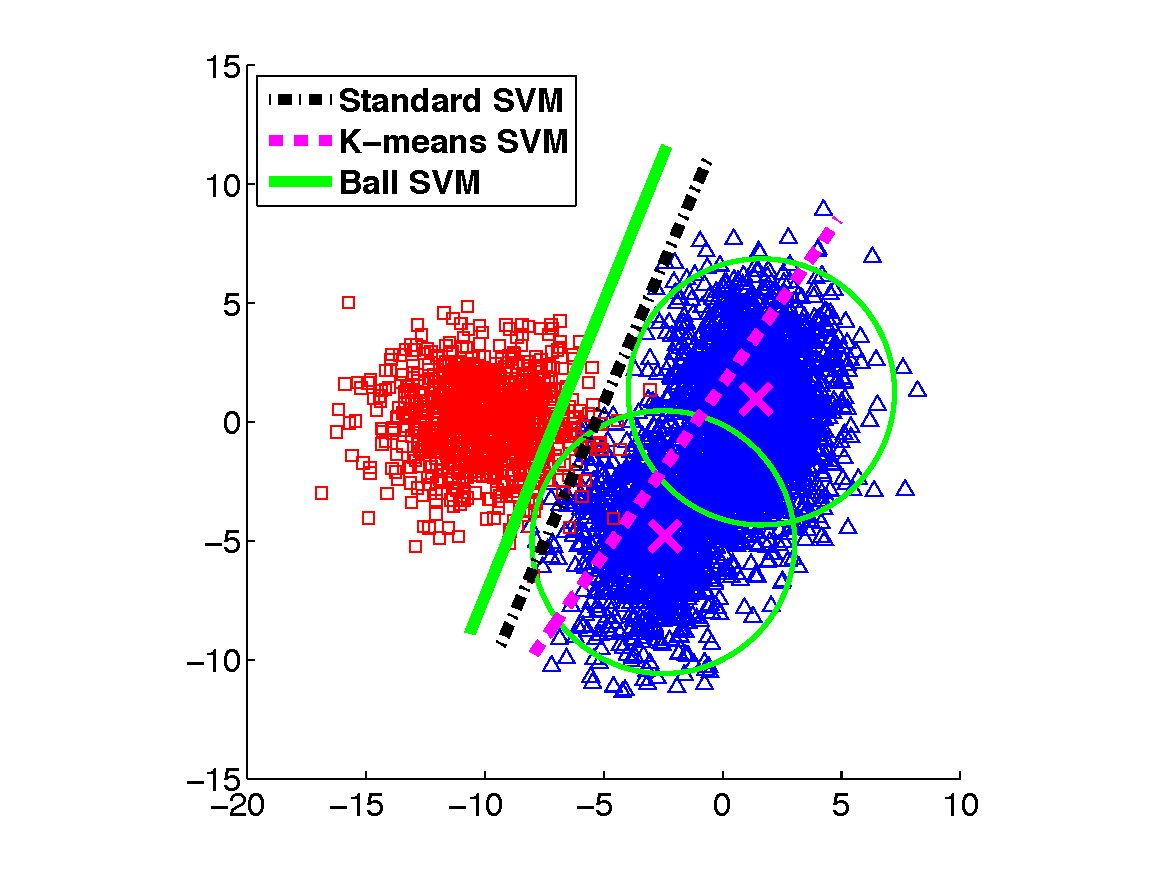
\includegraphics[scale = 0.4]{toy_neg_k_2.pdf}
}
\subfigure[$k=4$]{
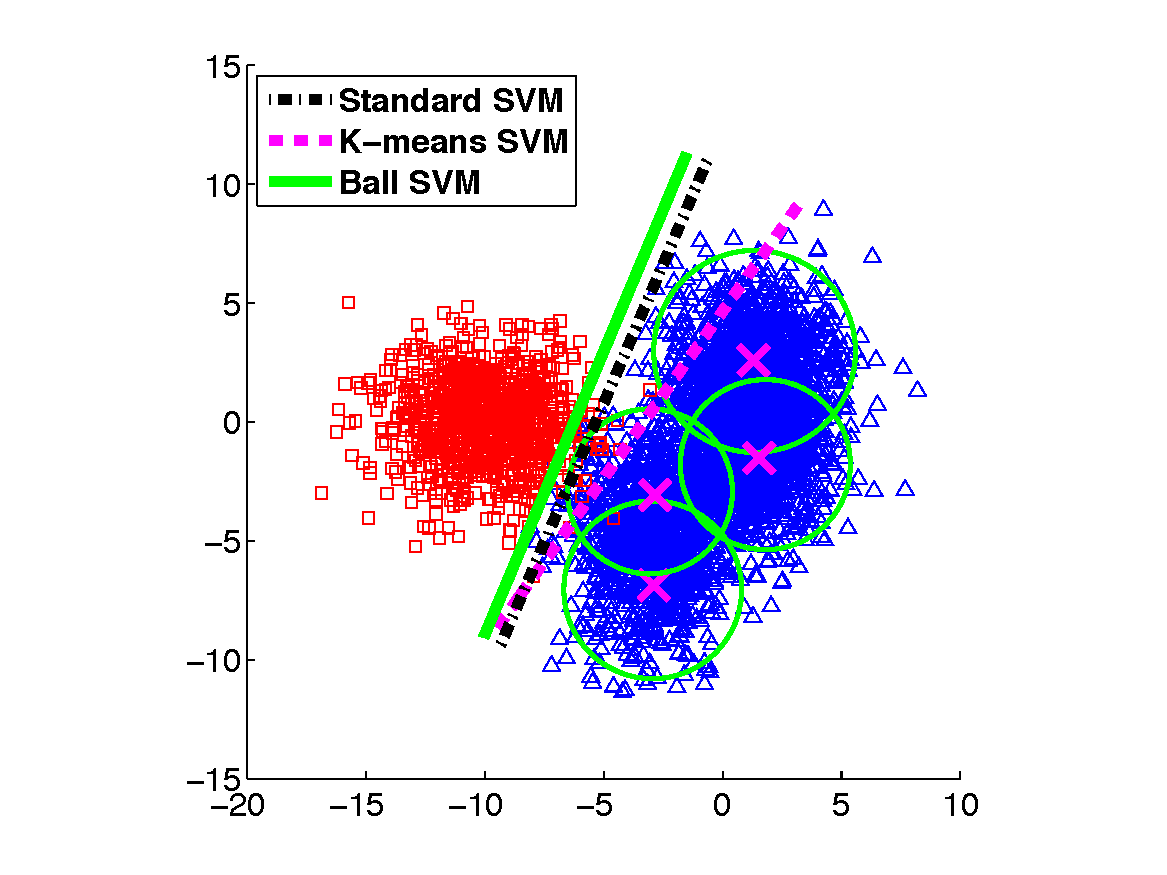
\includegraphics[scale = 0.4]{toy_neg_k_4.pdf}
}
\subfigure[$k=8$]{
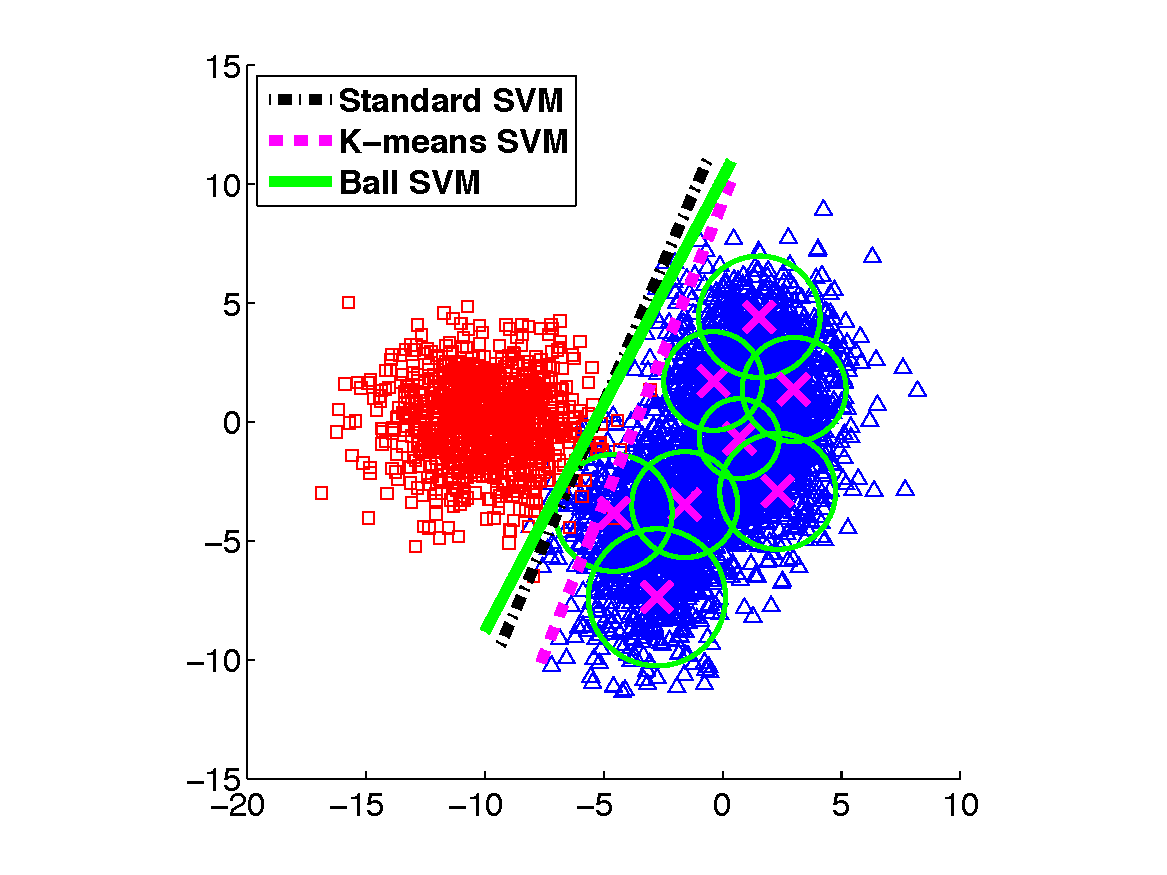
\includegraphics[scale = 0.4]{toy_neg_k_8.pdf}
}
\subfigure[$k=16$]{
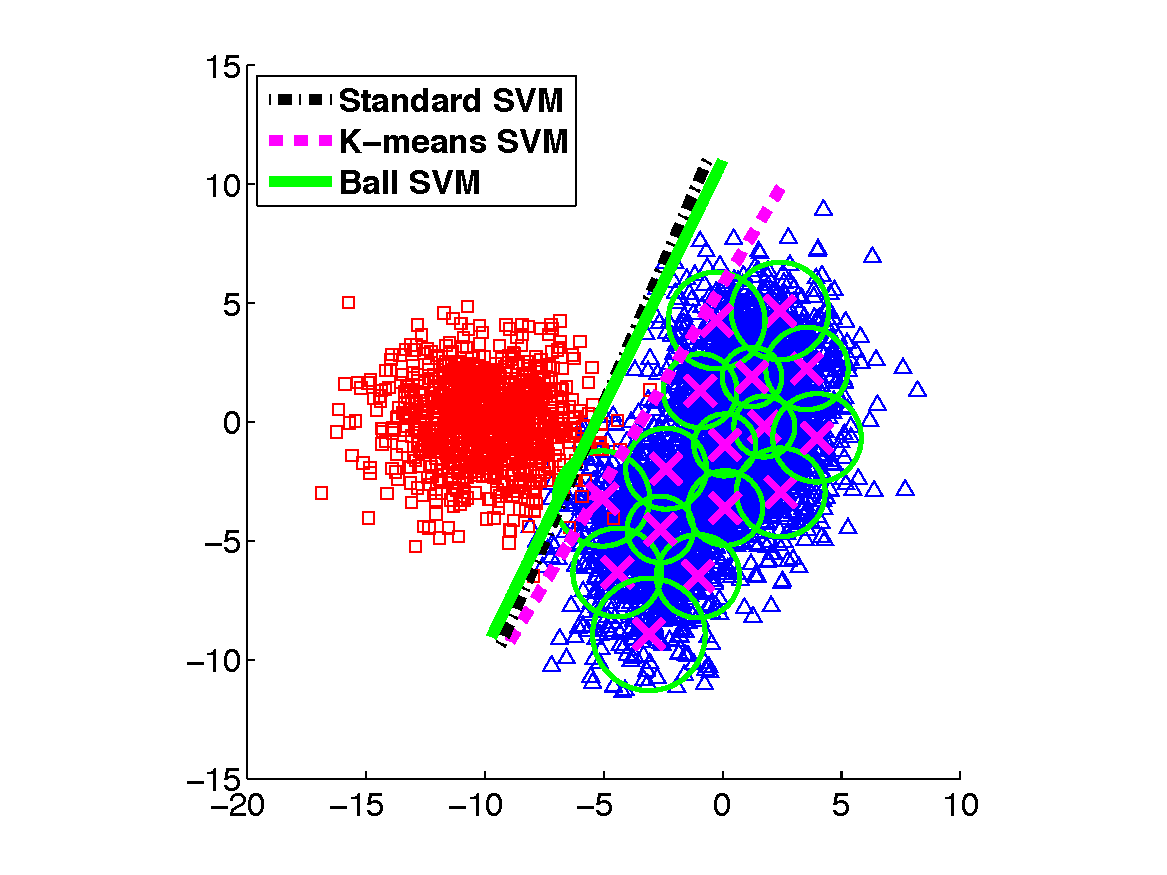
\includegraphics[scale = 0.4]{toy_neg_k_16.pdf}
}
\caption{Results on a toy 2D dataset.}~\label{fig:toy2d}
\end{figure}

\bibliographystyle{IEEEtran}
\bibliography{biblio}

\end{document}